\chapter{Data types in OpenGL}


\section{Basic types}
\label{sec:basic-types}

Like C, OpenGL also have intrinsic types. The difference is that these
types has the prefix \verb!GL!, as shown in Fig.~\ref{fig:types}.
\begin{verbatim}
GLint
GLuint
GLfloat 
GLenum
...
\end{verbatim}

\begin{figure}[hbt]
  \centerline{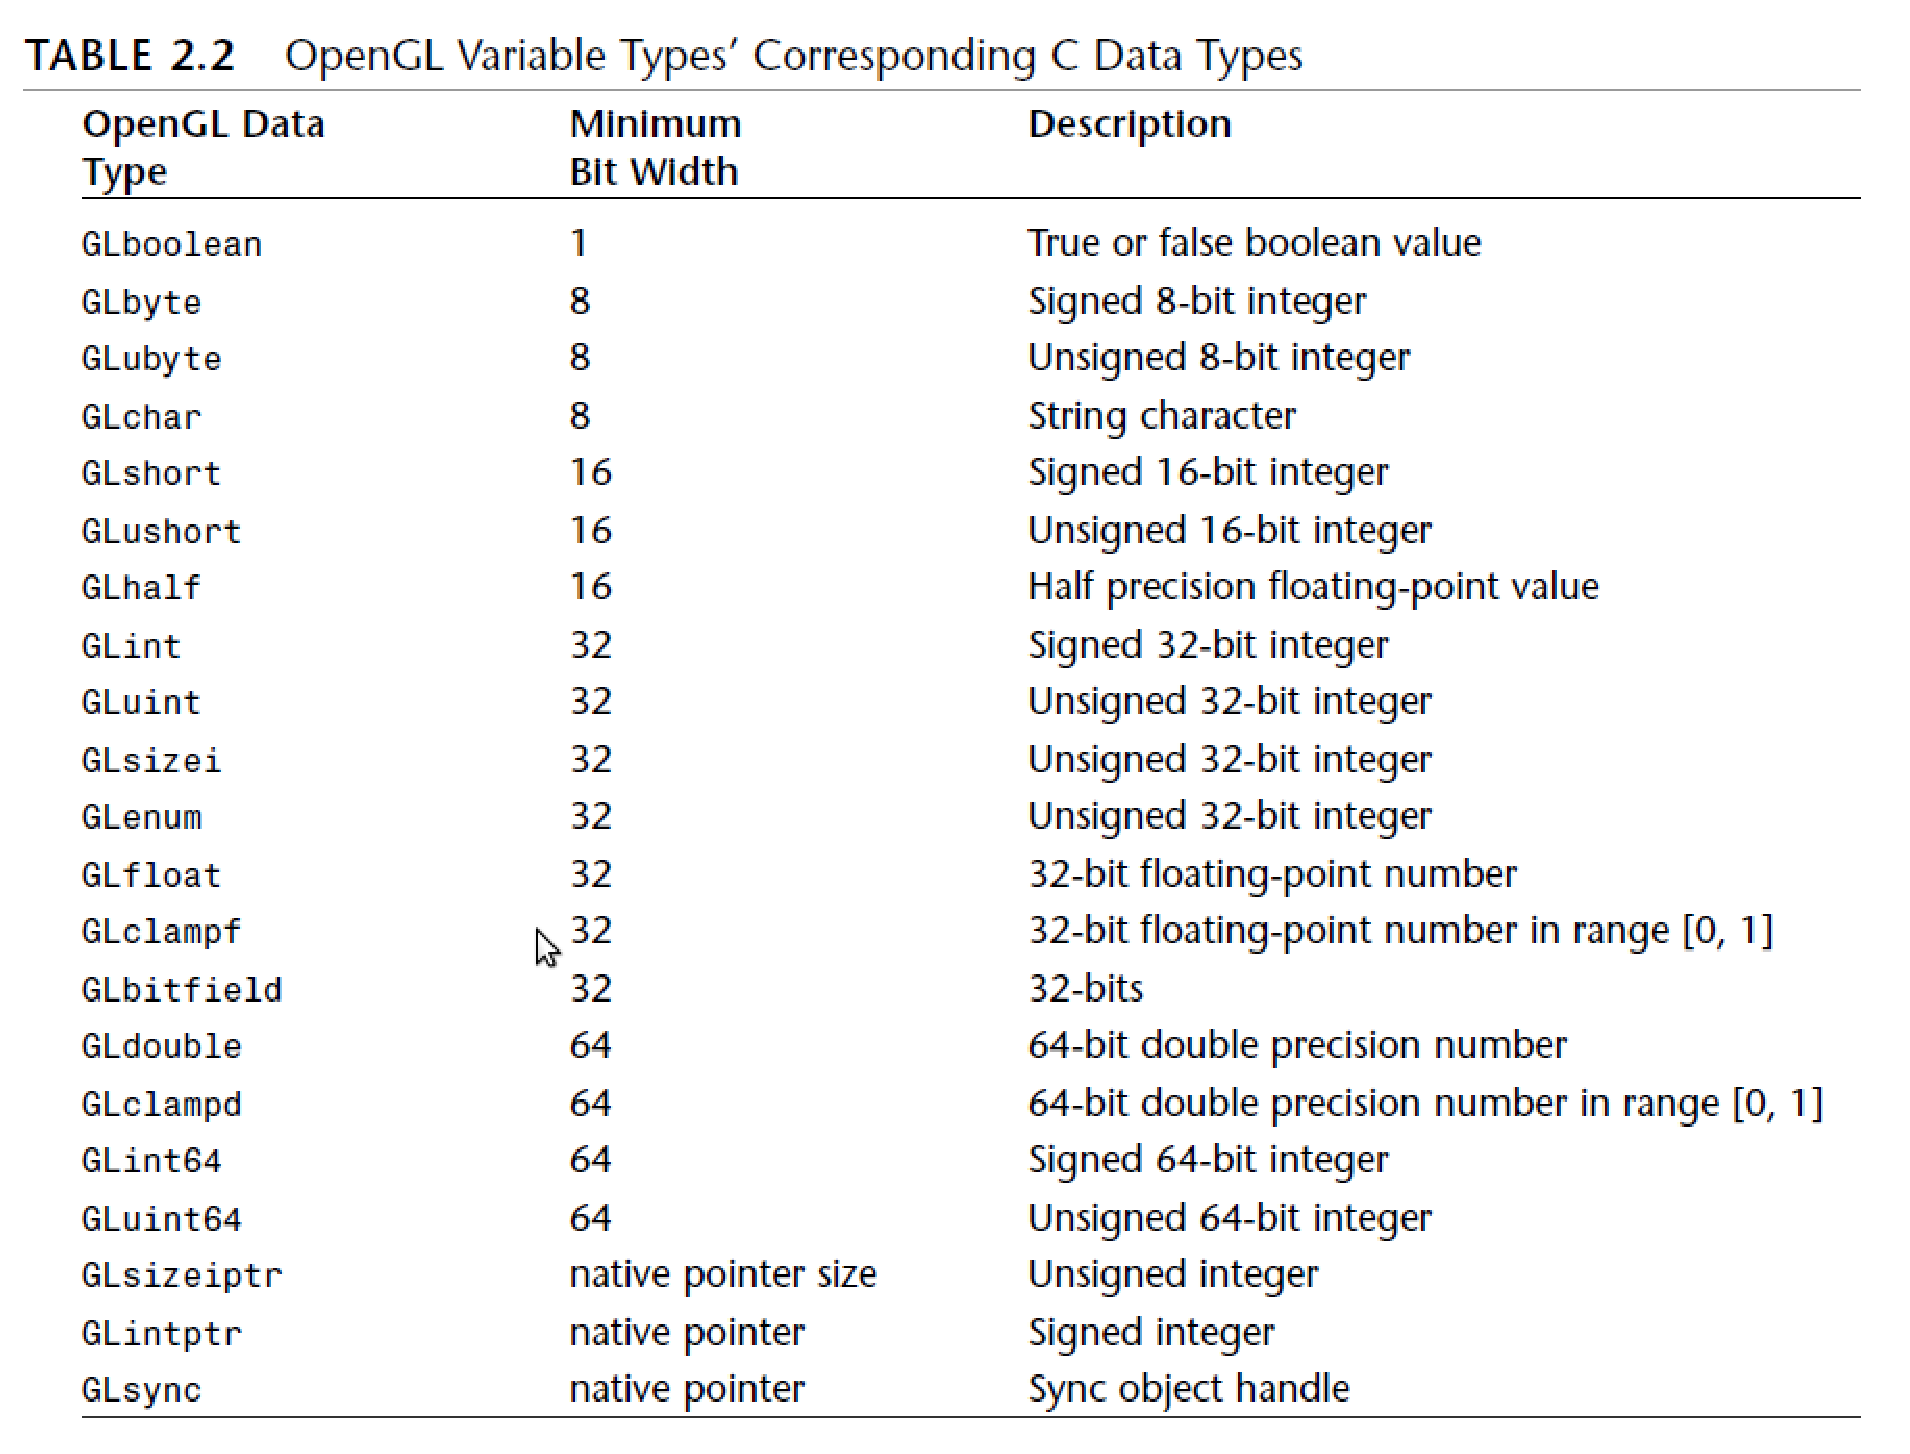
\includegraphics[height=10cm,
    angle=0]{./images/OpenGL_types.eps}}
  \caption{Basic types}
  \label{fig:types}
\end{figure}

The packed formats listed in Table \ref{tab:pixel_data_type} were
introduced in OpenGL 1.2 (and later) as a means of allowing image data
to be stored in a more compressed form that matched a range of color
graphics hardware. These are known as {\bf packed pixel format}. The
number of bits per color channels are shown in the constants

\begin{table}[hbt]
  \begin{center}
    \caption{Data Types for Pixel Data}
    \begin{tabular}{lp{6cm}} 
      \hline
      Constant & Description \\
      \verb!GL_UNSIGNED_BYTE! & Each color component is an 8-bit unsigned
      integer. \\
      \verb!GL_BYTE! & Signed 8-bit integer. \\
      \verb!GL_UNSIGNED_SHORT! & Unsigned 16-bit integer. \\
      \verb!GL_SHORT! & Signed 16-bit integer. \\
      \verb!GL_UNSIGNED_INT!& Unsigned 32-bit integer.\\
      \verb!GL_INT! & Signed 32-bit integer.\\
      \verb!GL_FLOAT!& Single-precision float.\\
      \verb!GL_HALF_FLOAT! & Half-precision float. \\
      \verb!GL_UNSIGNED_BYTE_3_2_2! & Packed RGB values.\\
      \verb!GL_UNSIGNED_BYTE_2_3_3_REV! & Packed RGB values.\\
      \verb!GL_UNSIGNED_SHORT_5_6_5! &Packed RGB values. \\
      \verb!GL_UNSIGNED_SHORT_5_6_5_REV!& Packed RGB values.\\
      \verb!GL_UNSIGNED_SHORT_4_4_4_4! &Packed RGBA values. \\
      \verb!GL_UNSIGNED_SHORT_4_4_4_4_REV!& Packed RGBA values. \\
      \verb!GL_UNSIGNED_SHORT_5_5_5_1!& Packed RGBA values.\\
      \verb!GL_UNSIGNED_SHORT_1_5_5_5_REV! & Packed RGBA values. \\
      \verb!GL_UNSIGNED_INT_8_8_8_8! & Packed RGBA values.\\
      \verb!GL_UNSIGNED_INT_8_8_8_8_REV! & Packed RGBA values. \\
      \verb!GL_UNSIGNED_INT_10_10_10_2! & Packed RGBA values.\\
      \verb!GL_UNSIGNED_INT_2_10_10_10_REV! & Packed RGBA values. \\
      \verb!GL_UNSIGNED_INT_24_8! & Packed RGBA values.\\
      \verb!GL_UNSIGNED_INT_10F_11F_11F_REV! & Packed RGBA values. \\
      \verb!GL_FLOAT_32_UNSIGNED_INT_24_8_REV! & Packed RGBA values \\
      \hline\hline
    \end{tabular}
  \end{center}
  \label{tab:pixel_data_type}
\end{table}


\section{Colors}
\label{sec:colors}

Fig.~\ref{fig:common_colors}

\begin{figure}[hbt]
  \centerline{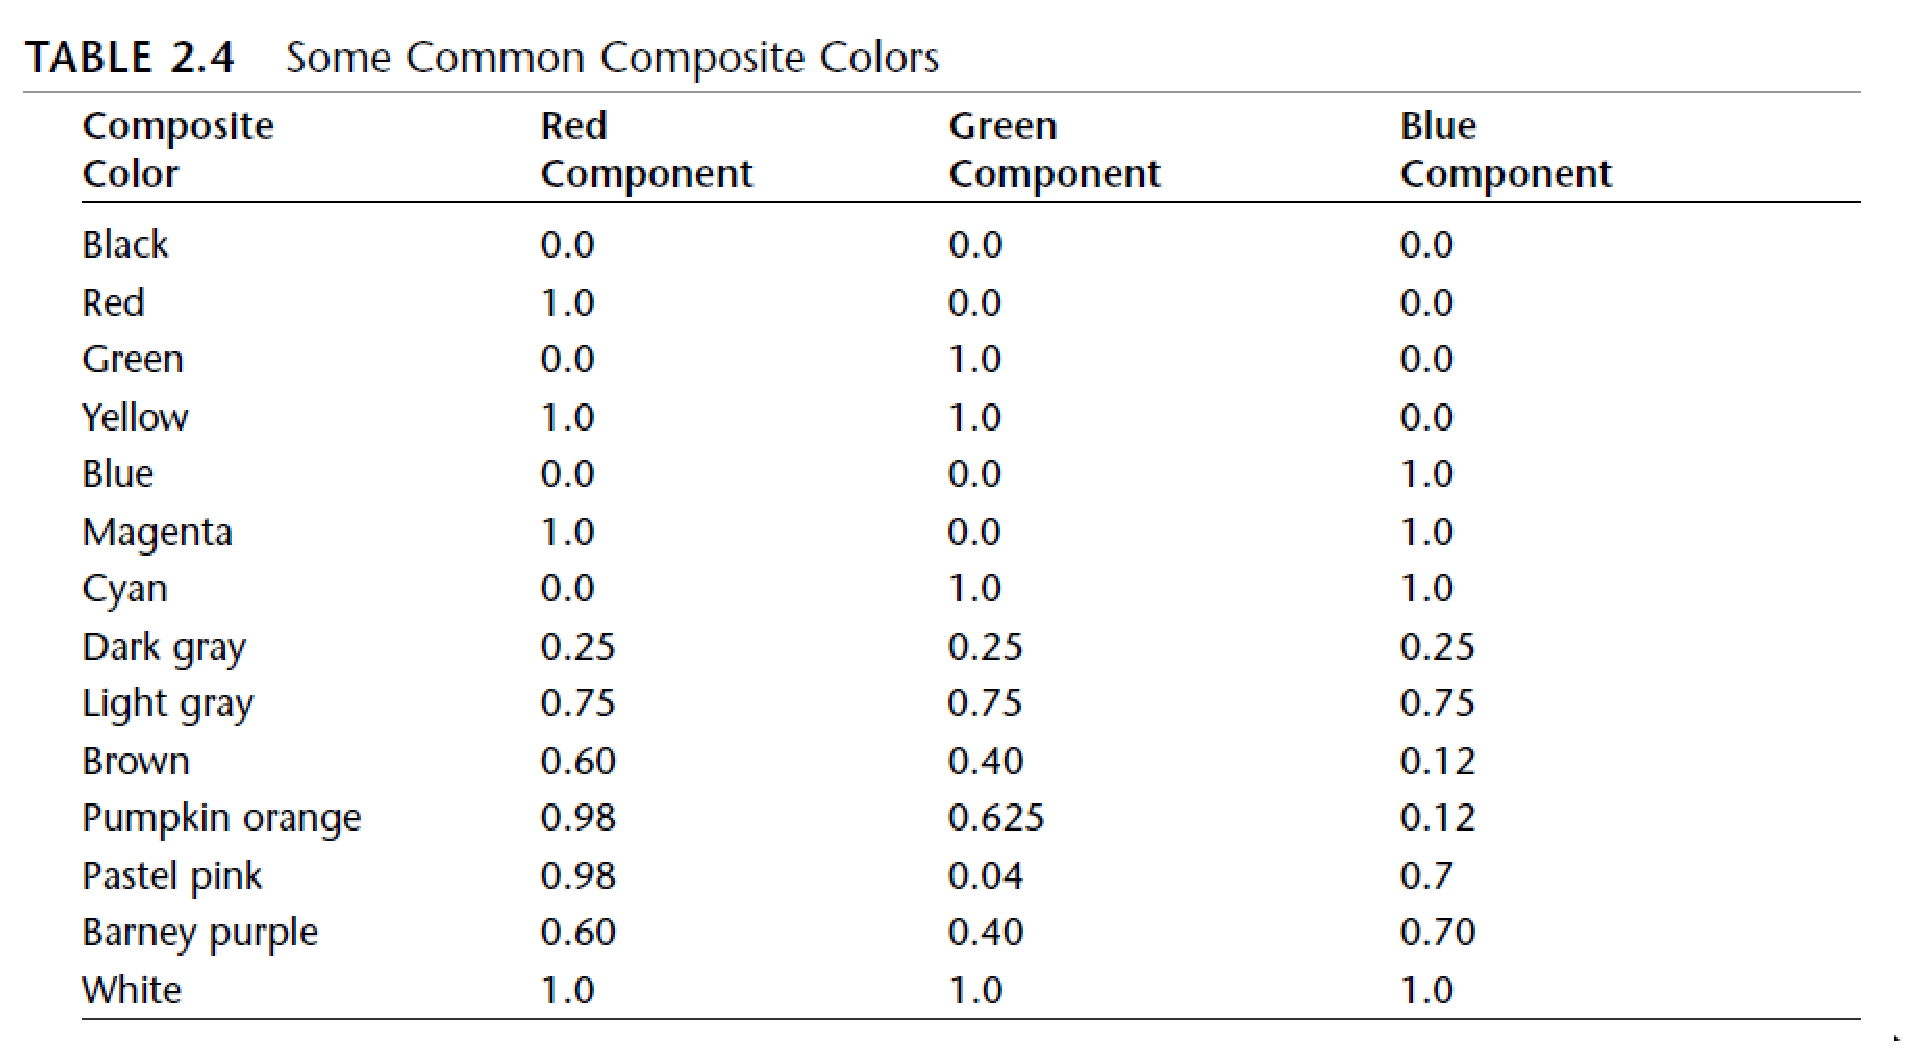
\includegraphics[height=8cm,
    angle=0]{./images/common_colors.eps}}
\caption{Common colors in OpenGL}
\label{fig:common_colors}
\end{figure}

Table~\ref{tab:OpenGL_color} in which the last three format
\begin{verbatim}
GL_STENCIL_INDEX, GL_DEPTH_COMPONENT, and GL_DEPTH_STENCIL
\end{verbatim}
are used for reading and writing directly to the stencil and depth
buffers.

\begin{table}[hbt]
  \begin{center}
    \caption{OpenGL pixel formats}
    \begin{tabular}{cp{9cm}} 
      \hline
      Constant & Description \\
      \verb!GL_RGB! & Colors are in red, green, blue order. \\
      \verb!GL_RGBA! & Colors are in red, green, blue, alpha order.\\
      \verb!GL_BGR!& Colors are in blue, green, red order.\\
      \verb!GL_BGRA!& Colors are in blue, green, red, alpha order.\\
      \verb!GL_RED!& Each pixel contains a single red component.\\
      \verb!GL_GREEN!& Each pixel contains a single green component.\\
      \verb!GL_BLUE!& Each pixel contains a single blue component.\\
      \verb!GL_RG!& Each pixel contains a red followed by a blue component.\\
      \verb!GL_RED_INTEGER!& Each pixel contains a red integer component.\\
      \verb!GL_GREEN_INTEGER!& Each pixel contains a green integer component.\\
      \verb!GL_BLUE_INTETER!& Each pixel contains a blue integer component.\\
      \verb!GL_RG_INTEGER!& Each pixel contains a red followed by a green integer component.\\
      \verb!GL_RGB_INTEGER!& Each pixel contains a red, green, and blue integer component, in
      that order.\\
      \verb!GL_RGBA_INTEGER! & Each pixel contains a red, green, blue, and alpha integer component,
      in that order.\\
      \verb!GL_BGR_INTEGER!& Each pixel contains a blue, green, and red integer component, in
      that order.\\
      \verb!GL_BGRA_INTEGER!& Each pixel contains a blue, green, red, and alpha integer component,
      in that order.\\
      \verb!GL_STENCIL_INDEX!& Each pixel contains a single stencil value.\\
      \verb!GL_DEPTH_COMPONENT!& Each pixel contains a single depth value.\\
      \verb!GL_DEPTH_STENCIL!& Each pixel contains a depth and a stencil value.\\
      \hline\hline
    \end{tabular}
  \end{center}
  \label{tab:OpenGL_color}
\end{table}


\section{Geometric Primitives}
\label{sec:primitives}

Given the vertices defined (Sect.~\ref{sec:attributes}), you now can
connect them to form complex geometric shapes. OpenGL has helped you
creating some basic shapes called primitives.

There are 10 primitives in OpenGL,
Table~\ref{tab:geometric_primitives}.

\begin{table}[hbt]
  \begin{center}
    \caption{OpenGL primitives\protect\footnotemark[1]}
    \footnotetext[1]{We now have: GL\_QUADS, GL\_QUAD\_STRIP,
      GL\_POLYGON}
    \begin{tabular}{cp{8cm}} 
      \hline
      Primitive &  Description\\
      \verb!GL_POINTS! & Each vertex is a single point on the screen. \\
      \verb!GL_LINES! &  Each pair of vertices defines a line segment. \\
      \verb!GL_LINE_STRIP! & A line segment is drawn from the first vertex to each successive vertex.\\
      \verb!GL_LINE_LOOP! & Same as \verb!GL_LINE_STRIP!, but the last and first
      vertex are connected. \\
      \verb!GL_TRIANGLES! & Every three vertices define a new triangle. \\
      \verb!GL_TRIANGLE_STRIP! & Triangles share vertices along a strip. \\
      \verb!GL_TRIANGLE_FAN! & Triangles fan out from an origin, sharing adjacent
      vertices.\\
      \hline\hline
    \end{tabular}
  \end{center}
  \label{tab:geometric_primitives}
\end{table}

% Besides using \verb!GL_POINTS!,
% i.e. each data element is a point, we can also use
% \begin{verbatim}
% GL_LINES, GL_LINE_STRIP, GL_LINE_LOOP,
% GL_TRIANGLES, GL_TRIANGLES_STRIP, GL_TRIANGLES_FAN,
% \end{verbatim}

\subsection{Points}
\label{sec:points}

By default, a point is just a single pixel on the screen. However, you
can change the point size
\begin{verbatim}
void glPointSize(GLfloat size);
\end{verbatim}
or
\begin{verbatim}
// enable the mode
glEnable(GL_PROGRAM_POINT_SIZE);

// and use shader built-in variable
gl_PointSize = 5.0; 
\end{verbatim}

As not all point sizes are supported, you use this to query
\begin{verbatim}
GLfloat sizes[2]; // Store supported point size range
GLfloat step; // Store supported point size increments

  // Get supported point size range and step size
glGetFloatv(GL_POINT_SIZE_RANGE,sizes);
glGetFloatv(GL_POINT_SIZE_GRANULARITY,&step);
\end{verbatim}

\begin{framed}
  The OpenGL specification requires only that one point size, 1.0, be
  supported, but most implementations support a wide range of point
  sizes.
\end{framed}

\subsection{Lines}
\label{sec:lines}

A batch of lines should consist of an even number of vertices.

Lines, by default, are one pixel in width. You can change using
\begin{verbatim}
void glLineWidth(GLfloat width);
\end{verbatim}

\subsection{Line strip}
\label{sec:line-strip}

\subsection{Line loop}
\label{sec:line-loop}

\subsection{Triangles}
\label{sec:triangles}

With 3 vertices, there are different ways of combination of order and
direction in which the vertices are specified to form the same
triangle. Each of combination is called {\bf winding}. The triangles
in Fig.~\ref{fig:winding} are said to have clockwise winding because they are
literally wound in the clockwise direction.

\begin{figure}[hbt]
  \centerline{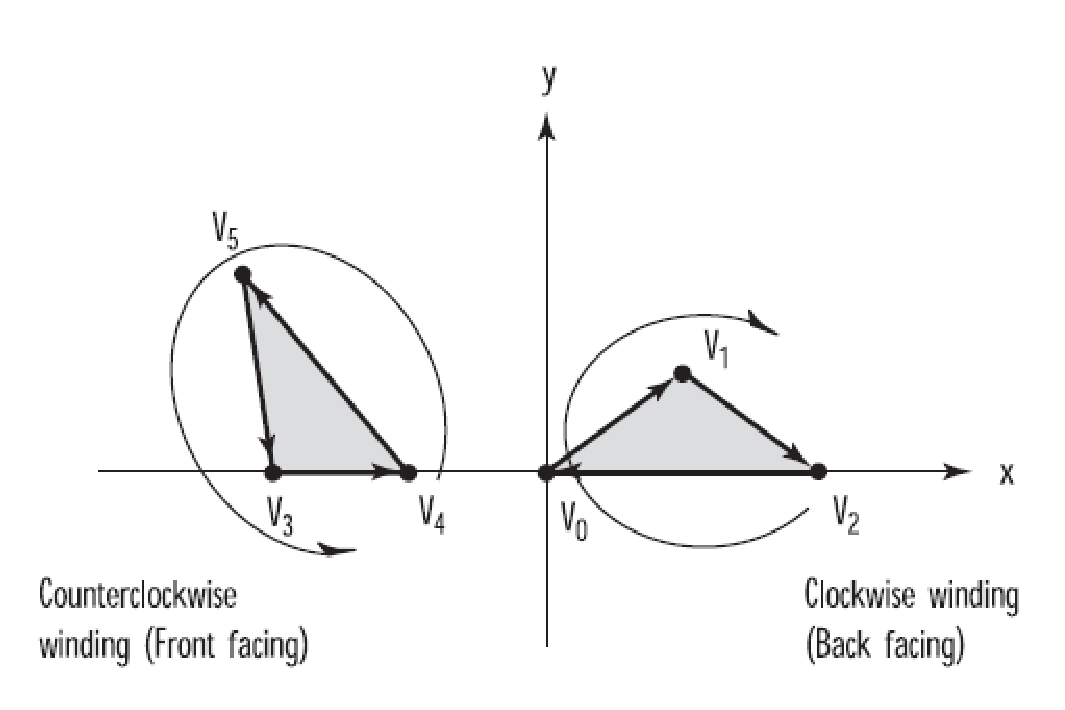
\includegraphics[height=5cm,
    angle=0]{./images/winding.eps}}
  \caption{Winding}
  \label{fig:winding}
\end{figure}

A 2D primitive, like a triangle, has 2 faces.  OpenGL, by default,
considers polygons that have counterclockwise winding to be front
facing. You can change, but make sure use the same convention for all
geometric shapes in your picture.
\begin{verbatim}
glFrontFace(GL_CW);   // or GL_CCW
\end{verbatim}

\begin{figure}[hbt]
  \centerline{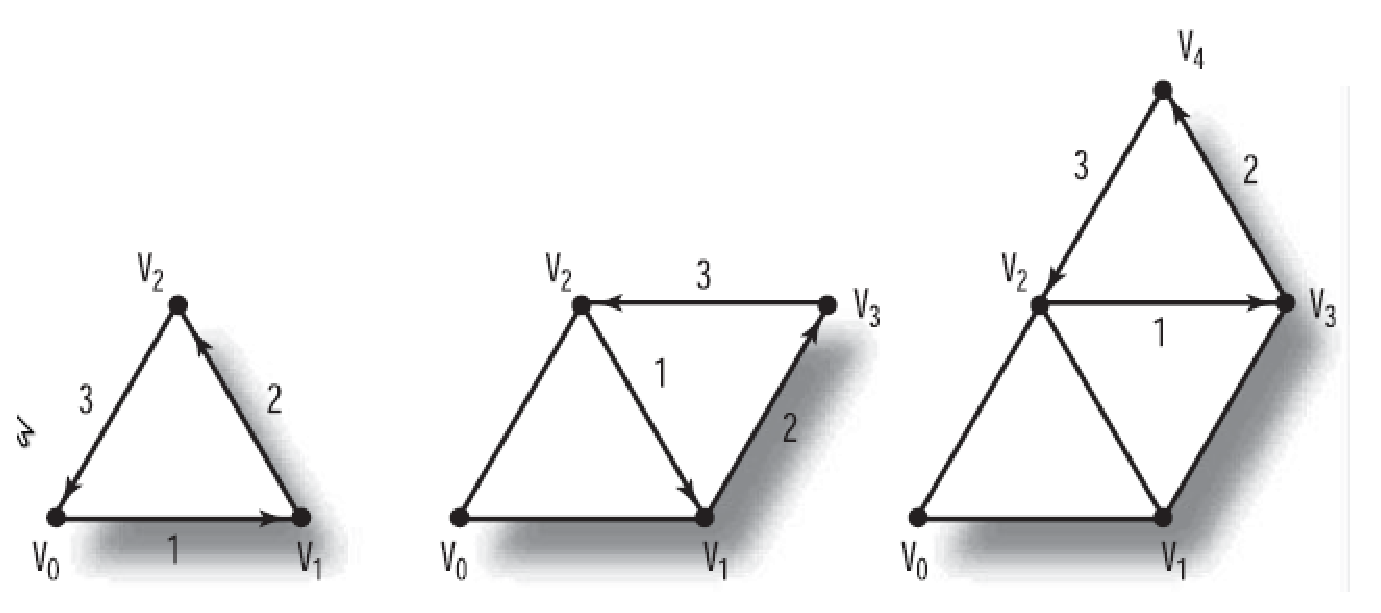
\includegraphics[height=5cm,
    angle=0]{./images/triangle_strip.eps}}
  \centerline{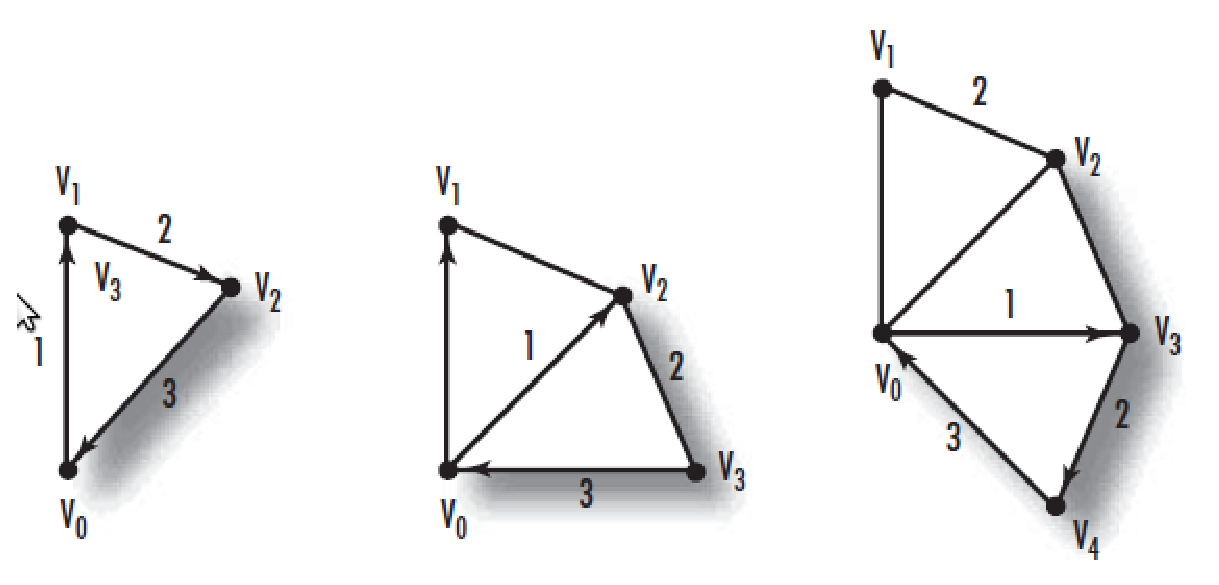
\includegraphics[height=5cm,
    angle=0]{./images/triangle_fan.eps}}

  \caption{(A) triangle strip, (B) triangle fan}
  \label{fig:triangle}
\end{figure}





